\chapter{Correctness}
\label{chap:correctness}

The Meteor authors have released a demo of Meteor at \cite{MeteorDemo2021}. There, they state that ``due to issues with the GPT-2 algorithm interface, you sometimes may see extra output from a decoded stegotext. This does not impact the underlying security of the scheme''.
During experimentation, I have concluded that the cause of this is due to the way sub-word based GNNs, such as GPT-2, represent text and not due to issues with the algorithm interface.

After describing the issue at hand, I will show that the Meteor Stegosystem is actually incorrect with respect to Hopper's definition as defined in \autoref{def:correctness-hopper} by providing a counterexample.
To restore correctness, I then present a change to Meteor's $Recover$ algorithm to successfully reconstruct the original hiddentext message while inducing overhead exponential in stegotext length.

\section{Ambiguous Tokenization}

In \autoref{sec:generative-neural-networks}, we discuss that GPT-2 uses a token dictionary to represent text.
To improve text generation and better recognize relations between words, sub-word tokenization might can words into sub-words.
Sub-word tokenization is opposed to word tokenization, which splits a text by spaces, and character-based tokenization, which tokenizes text character by character.
Sub-word tokenization allows for more flexible deep learning, as the framework can easier connect related words to each other. 
The model might learn that, by adding the suffix ``n't'' to a verb, one can invert the meaning of that verb, e.g. ``haven't'' is the opposite of ``have'' and those words are in close relation to each other.
This technique proves to be very effective in enhancing GNN performance.

On the other hand, this allows for one word to have multiple representations in the ML model.
For example, the word ``doesn't'' might be tokenized by a tokenizer $\mathcal{T}$ as $\mathcal{T}(\textrm{``doesn't''}) = ( \textrm{``do''}, \textrm{``es''}, \textrm{``n't''} )$. It could also be tokenized as $\mathcal{T}(\textrm{``doesn't''}) = ( \textrm{``does''}, \textrm{``n't''} )$ or even $\mathcal{T}(\textrm{``doesn't''}) = ( \textrm{``d''}, \textrm{``o''}, \textrm{``e''}, \textrm{``s''}, \textrm{``n''}, \textrm{``'t''})$.
This effect is what we call ambiguous tokenization.

\begin{definition}[Ambiguous Tokenization]
	Let $\mathcal{M}$ be a GNN with tokens $\mathcal{T} = \{ t_1, t_2, \dots, t_n \}$.
	We say that $\mathcal{M}$ has an ambiguous tokenizations, if there exists at least two ordered list of indices $I = (i, j, k, \dots), J = (q, r, s, \dots), I \neq J$ with $T_1 = t_i || t_j || t_k || \dots$ and $T_2 = t_q || t_r || t_s || \dots$ such that $t_I = t_J$.
\end{definition}

\section{Correctness Of The Meteor Stegosystem}

In \autoref{alg:decode}, we see that during decoding, the stegotext $c$ generated by \autoref{alg:encode} should be parsed as $c = \{c_0,c_1, \dots, c_{|c|-1|}\}$.
This task is performed by a tokenizer $\mathcal{T}$ associated with the underlying model.
Here, the $Decode$ algorithm expects that the parsing of $c$ can recover the originally generated $c_i$.
This unfortunately is, at least for the GPT-2 model, not the case for some combinations of stegotext, key and history.
In \autoref{sec:alg-rec-tok-candidates}, I show how to fix these correctness issues.

\begin{theorem}
The Meteor Stegosystem is not correct.
\end{theorem}

\begin{proof}
For Meteor to be correct, it must fulfil \autoref{def:correctness-kaptchuk}, i.e. for any $k \leftarrow KeyGen(1^\lambda)$ and hiddentext $m$:

$$\mathop{Pr}[Decode_{\mathcal{D}}(k, Encode_{\mathcal{D}}(k, m, \mathcal{H}), \mathcal{H}) = m] \geq 1 - \mathop{negl}(\lambda)$$

We show incorrectness by giving a counterexample. 
Let

\begin{lstlisting}[breaklines]
k = 0xb95e03a1d01b304f11dcf2bc844e5fd3cbed41253b0506876004207b2c2a10e
    2d89c1a40e93530bfcfaaee54e66ae048d2d2a536615b0a81afe792883877d5b6
m = 'Hello world'
H = 'Despite a long history of research and wide-spread applications to censorship resistant systems, practical steganographic systems capable of embedding messages into realistic communication distributions, like text, do not exist.\n\n'
\end{lstlisting}

The stegotext for these inputs when using the Meteor demo code is

\begin{lstlisting}
c = '\nZeus communication system, controlled by anÆ2 desktop mic with'
\end{lstlisting}

When passed to the standard GPT-2 Tokenizer, the substring ``Zeus'' of $c$ is parsed as \lstinline{['Z', 'eus']}, while the encoding process has generated ``Zeus'' with token sequence \lstinline{['Ze', 'us']}.
Therefore, the stegotext $c$ cannot be successfully decoded to the original hiddentext ``Hello world'', which violates correctness.
\end{proof}

After we have seen that this problem appears at least once by finding a counterexample, another question arises:
How often does this happen?
To approach this question, I have conducted an experiment which attempts to estimate the rate at which these incorrect decodings occur.
For that, I have repeatedly encoded the entire book of Hamlet in chunks of 1024 characters with random keys and histories of length 128 picked at random from Hamlet as well using a modified version of the Meteor demo code from \cite{MeteorDemo2021}.

The experiment shows that most stegotexts have at least one mismatch if they are of significant length.
When encoding 128 byte blocks, the probability to have no mismatched token sequences is about 0.55.
But when encoding larger blocks, that probability decreases to about 0.18.
Therefore, we have to find a way to deal with these failed decodings, especially if we plan to encode hiddentext messages of significant length.
In \autoref{sec:alg-rec-tok-candidates}, I present approaches to recover from decoding errors while introducing computational overhead exponential in stegotext length. 
In \autoref{chap:twowaycommunication}, I show how we can split the hiddentext message and use Microsoft's DialoGPT -- a derivation of GPT-2 -- to generate chat-like stegotext.
Splitting the hiddentext results in shorter stegotext, thus decreases the probability of tokenization mismatches.

\begin{figure}[htbp]%
	\begin{subfigure}{.5\textwidth}%
		\centering%
	    \resizebox{0.8\linewidth}{!}{%
			% This file was created with tikzplotlib v0.10.1.
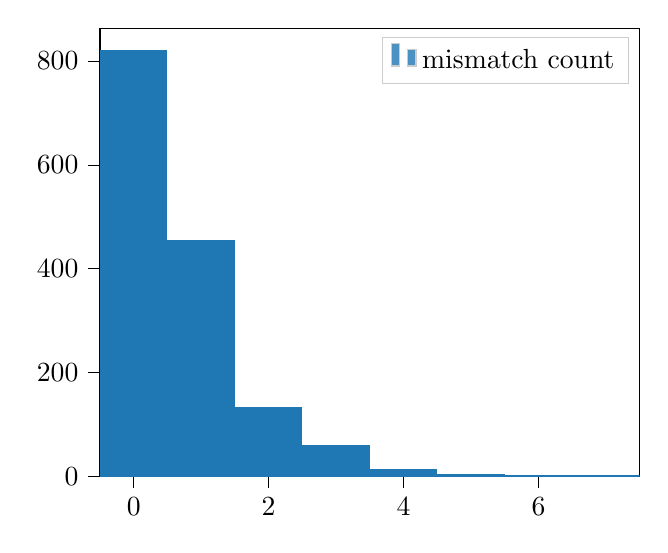
\begin{tikzpicture}

\definecolor{darkgray176}{RGB}{176,176,176}
\definecolor{lightgray204}{RGB}{204,204,204}
\definecolor{steelblue31119180}{RGB}{31,119,180}

\begin{axis}[
legend cell align={left},
legend style={fill opacity=0.8, draw opacity=1, text opacity=1, draw=lightgray204},
tick align=outside,
tick pos=left,
x grid style={darkgray176},
xmin=-0.5, xmax=7.5,
xtick style={color=black},
y grid style={darkgray176},
ymin=0, ymax=863.1,
ytick style={color=black}
]
\draw[draw=none,fill=steelblue31119180] (axis cs:-0.5,0) rectangle (axis cs:0.5,822);
\addlegendimage{ybar,ybar legend,draw=none,fill=steelblue31119180}
\addlegendentry{mismatch count}

\draw[draw=none,fill=steelblue31119180] (axis cs:0.5,0) rectangle (axis cs:1.5,455);
\draw[draw=none,fill=steelblue31119180] (axis cs:1.5,0) rectangle (axis cs:2.5,134);
\draw[draw=none,fill=steelblue31119180] (axis cs:2.5,0) rectangle (axis cs:3.5,61);
\draw[draw=none,fill=steelblue31119180] (axis cs:3.5,0) rectangle (axis cs:4.5,15);
\draw[draw=none,fill=steelblue31119180] (axis cs:4.5,0) rectangle (axis cs:5.5,5);
\draw[draw=none,fill=steelblue31119180] (axis cs:5.5,0) rectangle (axis cs:6.5,3);
\draw[draw=none,fill=steelblue31119180] (axis cs:6.5,0) rectangle (axis cs:7.5,3);
\end{axis}

\end{tikzpicture}
%
		}%
		\caption{128 bytes ($Pr[X=0] \approx 0.55$)}%
	\end{subfigure}%
	\begin{subfigure}{.5\textwidth}%
		\centering%
	    \resizebox{0.8\linewidth}{!}{%
			% This file was created with tikzplotlib v0.10.1.
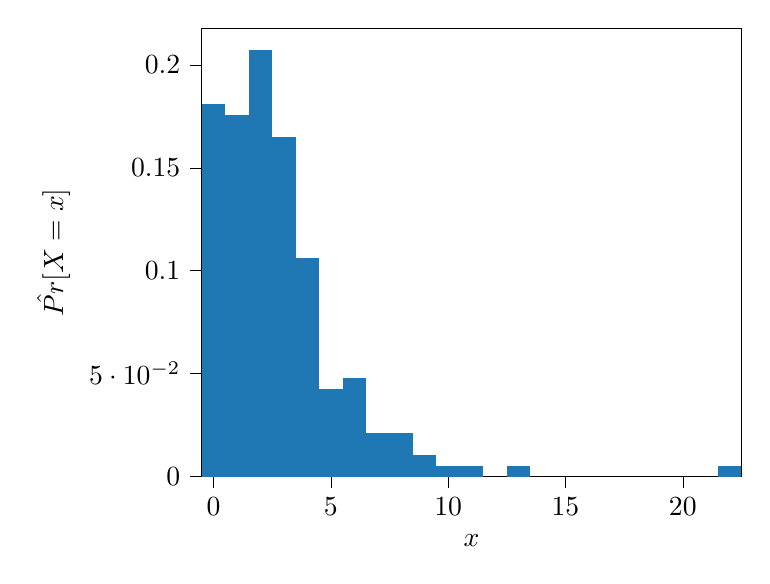
\begin{tikzpicture}

\definecolor{darkgray176}{RGB}{176,176,176}
\definecolor{steelblue31119180}{RGB}{31,119,180}

\begin{axis}[
tick align=outside,
tick pos=left,
x grid style={darkgray176},
xlabel={\(\displaystyle x\)},
xmin=-0.5, xmax=22.5,
xtick style={color=black},
y grid style={darkgray176},
ylabel={\(\displaystyle \hat{Pr}[X=x]\)},
ymin=0, ymax=0.21781914893617,
ytick style={color=black}
]
\draw[draw=none,fill=steelblue31119180] (axis cs:-0.5,0) rectangle (axis cs:0.5,0.180851063829787);
\draw[draw=none,fill=steelblue31119180] (axis cs:0.5,0) rectangle (axis cs:1.5,0.175531914893617);
\draw[draw=none,fill=steelblue31119180] (axis cs:1.5,0) rectangle (axis cs:2.5,0.207446808510638);
\draw[draw=none,fill=steelblue31119180] (axis cs:2.5,0) rectangle (axis cs:3.5,0.164893617021278);
\draw[draw=none,fill=steelblue31119180] (axis cs:3.5,0) rectangle (axis cs:4.5,0.106382978723405);
\draw[draw=none,fill=steelblue31119180] (axis cs:4.5,0) rectangle (axis cs:5.5,0.042553191489362);
\draw[draw=none,fill=steelblue31119180] (axis cs:5.5,0) rectangle (axis cs:6.5,0.0478723404255322);
\draw[draw=none,fill=steelblue31119180] (axis cs:6.5,0) rectangle (axis cs:7.5,0.021276595744681);
\draw[draw=none,fill=steelblue31119180] (axis cs:7.5,0) rectangle (axis cs:8.5,0.021276595744681);
\draw[draw=none,fill=steelblue31119180] (axis cs:8.5,0) rectangle (axis cs:9.5,0.0106382978723405);
\draw[draw=none,fill=steelblue31119180] (axis cs:9.5,0) rectangle (axis cs:10.5,0.00531914893617025);
\draw[draw=none,fill=steelblue31119180] (axis cs:10.5,0) rectangle (axis cs:11.5,0.00531914893617025);
\draw[draw=none,fill=steelblue31119180] (axis cs:11.5,0) rectangle (axis cs:12.5,0);
\draw[draw=none,fill=steelblue31119180] (axis cs:12.5,0) rectangle (axis cs:13.5,0.00531914893617025);
\draw[draw=none,fill=steelblue31119180] (axis cs:13.5,0) rectangle (axis cs:14.5,0);
\draw[draw=none,fill=steelblue31119180] (axis cs:14.5,0) rectangle (axis cs:15.5,0);
\draw[draw=none,fill=steelblue31119180] (axis cs:15.5,0) rectangle (axis cs:16.5,0);
\draw[draw=none,fill=steelblue31119180] (axis cs:16.5,0) rectangle (axis cs:17.5,0);
\draw[draw=none,fill=steelblue31119180] (axis cs:17.5,0) rectangle (axis cs:18.5,0);
\draw[draw=none,fill=steelblue31119180] (axis cs:18.5,0) rectangle (axis cs:19.5,0);
\draw[draw=none,fill=steelblue31119180] (axis cs:19.5,0) rectangle (axis cs:20.5,0);
\draw[draw=none,fill=steelblue31119180] (axis cs:20.5,0) rectangle (axis cs:21.5,0);
\draw[draw=none,fill=steelblue31119180] (axis cs:21.5,0) rectangle (axis cs:22.5,0.00531914893617025);
\end{axis}

\end{tikzpicture}
%
		}%
		\caption{1024 bytes ($Pr[X=0] \approx 0.18$)}%
	\end{subfigure}%
	\caption{Token mismatch statistic when using Meteor to encode Shakespear's Hamlet blockwise. The x-axis shows the number of tokenization mismatches between the encoding and the decoding party for hiddentext blocks with size...}
	\label{fig:meteor-stats-mismatch-count}	
\end{figure}

\section{Algorithmic Reconstruction Of Token Candidates}
\label{sec:alg-rec-tok-candidates}

Unfortunately, with sub-word tokenization, the decoding party cannot decide how the stegotext has been tokenized by the encoder.
To allow successful decoding of ambiguously tokenized stegotexts, I will in this section introduce algorithms to detect and fix wrong tokenizations. 


For that we have to modify the encoding step of Meteor to detect and fix wrong tokenization.
Before encoding, split the message $m$ into blocks $m_i$ of length $\gamma$.
After each block $m_i$, add a marker or checksum $q_i = q(m_i)$ of length $\delta$ into the hiddentext, i.e. $q \colon \{ 0,1 \}^\gamma \rightarrow \{ 0,1 \}^\delta$.
This marker helps the decoder to decide if the decoding is still correct up to this point.
The marker $q_i$ can be a checksum of $m_i$ or a fixed marker.
By using markers, we introduce $\delta \cdot \frac{|m|}{\gamma}$ bits of overhead to the hiddentext.
The modified $Encode$ algorithm can be found at \autoref{alg:marked-encode}.

Now the decoding party has to verify that after each block $m_i$ of $\gamma$ bits, the marker $q(m_i)$ appears and is valid.
If not, a decoding error has occured in the stegotext.
The modified $Decode$ algorithm can be seen at \autoref{alg:marked-decode}.

\begin{Pseudocode}[float, caption={Marked Encode Algorithm}, label={alg:marked-encode}]
algorithm $MarkedEncode_{\mathcal{M}}^{\beta, \gamma}(k_{prg}, m, \mathcal{H}, q)$
	Output: Stegotext message $c$
	$c \leftarrow \epsilon,~ n \leftarrow 0$
	$m^* \leftarrow \epsilon,~ j \leftarrow 0$
	while $j < |m|$ do
		$m^* \leftarrow m^* || m_j$
		$j \leftarrow j + 1$
		if $j \equiv 0~ \pmod \gamma$
			$m^* \leftarrow m^* || q(m_j)$
	while $n < |m^*|$ do
		$mask \leftarrow PRG.Next(k_{prg})$
		$r \leftarrow m^*[n:n+\beta] \oplus mask$
		$c_i \leftarrow Sample_{\mathcal{M}}^\beta(\mathcal{H}, r)$
		$\mathcal{R} = Recover_{\mathcal{M}}^\beta(\mathcal{H}, c_i)$
		$n_i \leftarrow LenPrefix^\beta(\mathcal{R})$
		$c \leftarrow c || c_i, n \leftarrow n+n_i, \mathcal{H} \leftarrow \mathcal{H}||c_i$
	Output $c$
\end{Pseudocode}



\begin{Pseudocode}[float, caption={Marked Decode Algorithm}, label={alg:marked-decode}]
algorithm $MarkedDecode_{\mathcal{M}}^{\beta,\gamma}(k_{prg}, c, \mathcal{H}, q)$
	Output: Plaintext message $m$
	$m \leftarrow \epsilon,~ n \leftarrow 0,~ j \leftarrow 0$
	Parse $c$ as $\{ c_0, c_1, \dots, c_{|c|-1} \}$
	for $i \in \{0, 1, \dots, |c|-1 \}$ do
		$\mathcal{R} = Recover_{\mathcal{M}}^\beta(\mathcal{H}, c_i)$
		$n_i \leftarrow LenPrefix^\beta(\mathcal{R})$
		$n \leftarrow n + n_i$
		$j \leftarrow j + n_i$
		if $j \geq \gamma$
			$j \leftarrow j - \gamma$
			!!TODO!! fixme n is wrong here, need to track current index
			if $m[n:n+\gamma] \neq q(m_i)$ do
				rollback()
		$m_i \leftarrow Prefix^\beta(\mathcal{R})$
		$mask \leftarrow PRG.Next(k_{prg})$
		$m \leftarrow m || (m_i \oplus mask[0: |m_i|])$
		$\mathcal{H} \leftarrow \mathcal{H}||c_i$
	Output $m$
\end{Pseudocode}
\todo{Modify Decode to MarkedDecode}

For the modification above, we need a helper algorithm which generates all possible tokenizations for a given stegotext.
We can represent these tokenization candidates in a graph using the ML models's tokens $\mathcal{T}$.

When passed a string $c$, the algorithm \emph{TokenizeCandidates} generates a directed, acyclic graph (DAG) $G = (V, E)$.
The nodes $v \in V$ represent all possible suffix strings of $c$ with $|V| = |c| + 1$.
The edges $e \in E$ represent possible tokens to use to transition between suffixes.
An example graph for input ``hello'' can be found at \ref{fig:ex-graph-tokenize-candidates}.
For example, the suffix string ``ello'' can be transformed to ``lo'' by removing the token ``el''.

Now that we have a graph for $c$, we can generate every possible sequence of tokens which $c$ can be parsed as.
For that, we use the algorithm $AllPaths$, which takes as input a graph $G = (V, E)$ and a start node $v_i \in V$ and returns a set of all possible paths between $v_i$ and a sink node $v_j = \epsilon$.

But how many paths exist between $v_i$ and $v_j$? A path between $v_i$ and $v_j$ is a subset of $E$ which contains both $v_i$ and $v_j$.
In the worst case, $G$ is a DAG with $\frac{n(n-1)}{2}$ edges and $v_i = max_{topological}(V)$ and $v_j = min_{topological}(V)$.
There are at most $2^{|V|-2} = 2^{|c|-1}$ subsets of $E$ which contain both $v_i$ and $v_j$.
The output of $AllPaths$ is exponential in input length.
A DFS-based implementation for AllPaths can be found at \autoref{alg:all-paths}.

\begin{Pseudocode}[float,caption={TokenizeCandidates algorithm},label={alg:tokenize-candidates}]
	algorithm $TokenizeCandidates_{\mathcal{T}}(s)$
		Output: Graph $G = (V, E)$
		if $s = \epsilon$
			return $\epsilon$
		for $t \in \mathcal{T}$ do
			if $s[0{:}|t|] = t$ do
				$V \leftarrow V \cup \{ s[|t|{:}] \}$
				$E \leftarrow E \cup \{ (s, s[|t|{:}]) \}$
				$G \leftarrow G \cup TokenizeCandidates_{\mathcal{T}}(s[|t|{:}])$
		return $G$
\end{Pseudocode}

\begin{figure}[htbp]
	\centering
	\begin{tikzpicture}
		\node[block] (hello) {hello};
		\node[block, right=15mm of hello] (lo) {lo};
		\node[block, above=15mm of lo] (llo) {llo};
		\node[block, above=15mm of llo] (ello) {ello};
		\node[block, below=15mm of lo] (o) {o};
		\node[block, right=15mm of lo] (bot) {$\epsilon$};
		
		\draw[->] (hello) to node[above] {h} (ello);
		\draw[->] (hello) to node[above] {he} (llo);
		\draw[->] (hello) to node[above] {hel} (lo);
		\draw[->] (hello) to node[left] {hell} (o);
		\draw[->, bend right=120] (hello) to node[below] {hello} (bot);

		\draw[->] (ello) to node[right] {e} (llo);
		\draw[->, bend left=30] (ello) to node[right] {el} (lo);
		\draw[->, bend left=30] (ello) to node[above] {ell} (o);
		\draw[->] (ello) to node[right] {ello} (bot);

		\draw[->] (llo) to node[right] {l} (lo);
		\draw[->, bend right=30] (llo) to node[above] {ll} (o);
		\draw[->] (llo)   to node[above] {llo} (bot);

		\draw[->] (lo)    to node[right] {l} (o);
		\draw[->] (lo)    to node[above] {lo} (bot);

		\draw[->] (o)     to node[above] {o} (bot);
	\end{tikzpicture}
	\caption{Graph generated by $TokenizeCandidates_{\mathcal{T}}(``hello'')$ with $\mathcal{T} = \{ h, e, l, l, o, el, he, ll, lo, ell, hel, llo, hell, ello, hello \}$}
	\label{fig:ex-graph-tokenize-candidates}
\end{figure}
\todo{improve tikz graph}

\begin{Pseudocode}[float,caption={DFS-based algorithm which generates a list of all possible paths between between two nodes in a DAG},label={alg:all-paths}]
algorithm $AllPaths(G, root, sink)	$
	Output: List of paths between $root$ and $sink$
	if $root = sink$ do
		return $[[\bot]]$
	$queue \leftarrow \epsilon$
	$paths \leftarrow []$
	$hops \leftarrow OutEdges(G, root)$
	$queue \leftarrow queue + hops$
	for $hop \in hops$ do
		$subpaths \leftarrow AllPaths(G, hop, sink)$
		for $subpath \in subpaths$ do
			$paths \leftarrow [[root] + subpath]$
	return $paths$
\end{Pseudocode}
\todo{improve performance using dynamic programming}